\documentclass[10pt,conference,compsocconf]{IEEEtran}

\usepackage{hyperref}
\usepackage{graphicx}	% For figure environment

\begin{document}
\title{The Higgs Boson: A Tentative Prediction Model}

\author{
  Reynaud Alexandre, Sqalli Houssaini Othmane, Cloux Olivier\\
  \textit{Department of Computer Science, EPFL, Switzerland}
}

\maketitle

\begin{abstract}
The Higgs boson is an elementary particle in the standard model of physics which explains why other particles have mass. As it's impossible to observe directly, we observe the ``decay signature'' produced when two protons are smashed against one another. We present here a revolutionary method that will allow us to ``observe'' Higgs bosons through their signature.
\end{abstract}

\section{Introduction}
Since the dawn of humanity, a question sticked around: if I break this thing, what's inside? This led to many discoveries, including protons, neutrons. These are made of elementary particles\cite{elementPart}, among which are bosons, a particle that partly explains why particles have mass. Peter Higgs (among others) proposed the mechanism that explains it, that implies the existence of this boson.

But observing it directly is hard. The best method out there is to smash two protons against one another, and observe the resulting decay, called the signature.

In this project, we conjecture that the behavior of the Higgs Boson is deterministic, and that it's behavior can be consequentially predicted. We will try to model such behavior to try and substantiate our claim. For that, we separate the set of observed data, and try to fit a model to the training set. If we can correctly (or at least with an acceptable accuracy) determine which of the remaining data (the test set) are Higgs bosons, then we will be confident that the aforementioned behavior is deterministic.

A lot of the physic background is taken from \cite{higgsBoson}.
\section{Models And Methods}
The complete pipeline of our methods is summarized in figure \ref{fig:my_label}.
\begin{figure*}
    \centering
    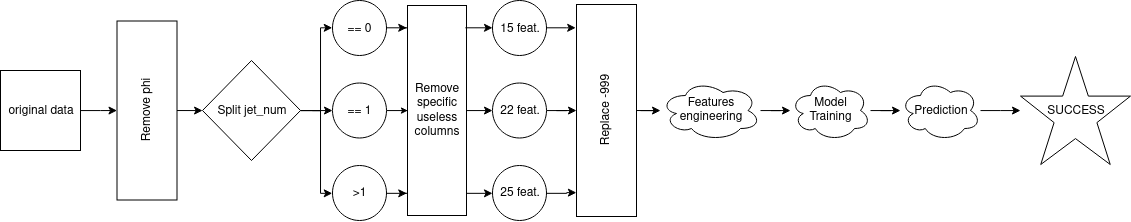
\includegraphics[scale=0.45]{pipeline.png}
    \caption{Complete pipeline}
    \label{fig:my_label}
\end{figure*}
\subsection{Methods}
\subsubsection{Preprocessing}
Multiple shortcomings can be encountered  in the data, meaning preprocessing is necessary before any modeling can be performed.
These are the forms they take and how they're dealt with:
\begin{itemize}
\item Uncorrelated Attributes: Three of the attributes "PRI\_tau\_phi", "PRI\_lep\_phi" and "PRI\_met\_phi" behave oddly.
  The distribution of these attributes shows a lack of causation between them and the type of the corresponding particle. This makes them irrelevant in the context of our pursuit, they are dropped to reduce noise and spare computational power.
\item Multiple Distributions: Attributes with an unexpectedly large amount of invalid values (-999) can be observed. By plotting the distribution of said attributes for each categorical value of "jet\_num", one can observe that the unwanted elements are absent for some values of "jet\_num" and are the only elements for some others. This makes it clear that the attribute is only meaningful for certain values of "jet\_num".To solve this problem, we split the dataset into 3 sub-samples (for "jet\_num"= 0,1,\{2,3\}) so that each distribution can be modeled separately, meaningless attributes are then dropped.
\item Measurement Errors: After the previous steps, some unwanted values remain and are so few and far between that it is reasonable to treat them as measurement errors. To prevent them from having an unwanted effect without dropping the corresponding sample, they are set to the most frequent value taken by the corresponding attribute.
\end{itemize}
\subsubsection{Augmentation}
The tools at our disposition are "Logistic Regression", "Least Squares" and variants, in other words, linear models. The phenomenon to model being far from trivial, it is a necessity to introduce non-linearities to obtain more than a weak classifier. To obtain said non-linearities, we expand our list of attributes through the following transformations:
\begin{enumerate}
    \item For all sets of different attributes \{x1,...xk\} of maximum size d0:
    \newline
    x1,...,xk $\rightarrow$ x1*...*xk
    \item For all attributes x and powers d1 $> 1$: 
    \newline
    $x \rightarrow x^{d1}$
    \item For all attributes x and powers d2 $\geq 1$: 
    \newline
    $x \rightarrow tanh(x)^{d2}$
    \item For all attributes x and powers d3 $\geq 1$: 
    \newline
    $x \rightarrow invlog(x)^{d3}$
    \item For all attributes x and powers d4 $\geq 1$:
    \newline
    $x \rightarrow x^{1/d4}$
\end{enumerate}
These were inspired by scientific documentation attached to the phenomenon to modelize. In order to let room for optimization, d0, d1, d2,d3 and d4 are set independently and consequently don't have to share the same value.


\subsection{Model}
\subsubsection{Model Selection}
After preprocessing and doing feature engineering to our data, it's now time to choose a model to start the training process.


As we now have 3 subsets of data we run multiples combinations of machine learning methods. Least Squares performed well and gave good results but we eventually chose to train all 3 subsets with the Ridge Regression method independently of each other to obtain a more optimized version of our least squares model through the selection of the hyper-parameter lambda.
\subsubsection{Hyper-parameter Selection}
 As we have three different subsets, it is clear that in order to get the best results we need to train each subset with different hyper-parameters.
 
 With Ridge Regression, we have only one hyper-parameter $\lambda $. We used a grid search in a power 10 space for each subset and measured the accuracy to find the best $\lambda $ for that subset.
 The following table shows the optimal hyper-parameters we have obtained.
 \vspace{3mm}

\begin{tabular}[c]{|l||l|l|l|l|l|l|l|}
\hline
d0&d1&d2&d3&d4&lambda1&lambda2&lambda3\\
\hline
3&3&3&3&3&2.26e-15&0&2.21e-16
\end{tabular}
\vspace{3mm}

To estimate the lambdas viably, we use basic 80/20 split cross-validation.  
Then, in order to validate the efficiency of our model, we apply a k-fold cross validation, splitting our training set into k-1 subsets for training and 1 subset for validation. In this project we choose a value of 5 for k.
\section{Results}
A non-deterministic process could not be predicted with more than a 50\% accuracy as there are only two possible outcomes.
Given that our model has consistently obtained an accuracy of more than 80 \% (82\% on aicrowd),we can reasonably conclude that the studied phenomenon is deterministic.
\section{Discussion}
We modeled the behavior of the Higgs Boson through Ridge Regression. Such a model showed many advantages:
\begin{itemize}
\item Interpretability: Being linear, our model can take the form of a mathematical equation making it simple to read and understand. 
\item Simplicity: The algorithm we use doesn't require much processing power, making it simpler to use and optimize (testing many hyper-parameters is viable).
\end{itemize}
However, it also comes with its share of shortcomings:
\begin{itemize}
\item Pseudo Non-Linearity: Our model is linear and non-linearities can only be injected in a incomplete way, making expressivity of our model insufficient. 
\item Prior Knowledge Requirements: Non-linearities must be manually added, making a good understanding of the phenomenon to model compulsory for the choice of said functions to be truly meaningful.
\end{itemize}
Ultimately, our model allows to support the determinism of the Higgs Boson and somewhat predict it's behavior. 
\section{Summary}
To conclude, the results we obtained back up our original claim and even allow us to predict with a decent accuracy the presence of a Higgs Boson.We conjecture that the lack of absolute determinism is due to the limited expressivity of our model and the insufficiencies of the information available for training. Scientists can take advantage of the interpretability of our model to try and understand the phenomenon at hand, but further investigation is highly encouraged.

\bibliographystyle{IEEEtran}
\bibliography{literature}

\end{document}